\chapter{Measurement Campaign}
\section{Setup}
The setup of the measurement will give the insight and solutions to the problems hypothesised in previous chapters. 

\begin{figure}[H]
\centering
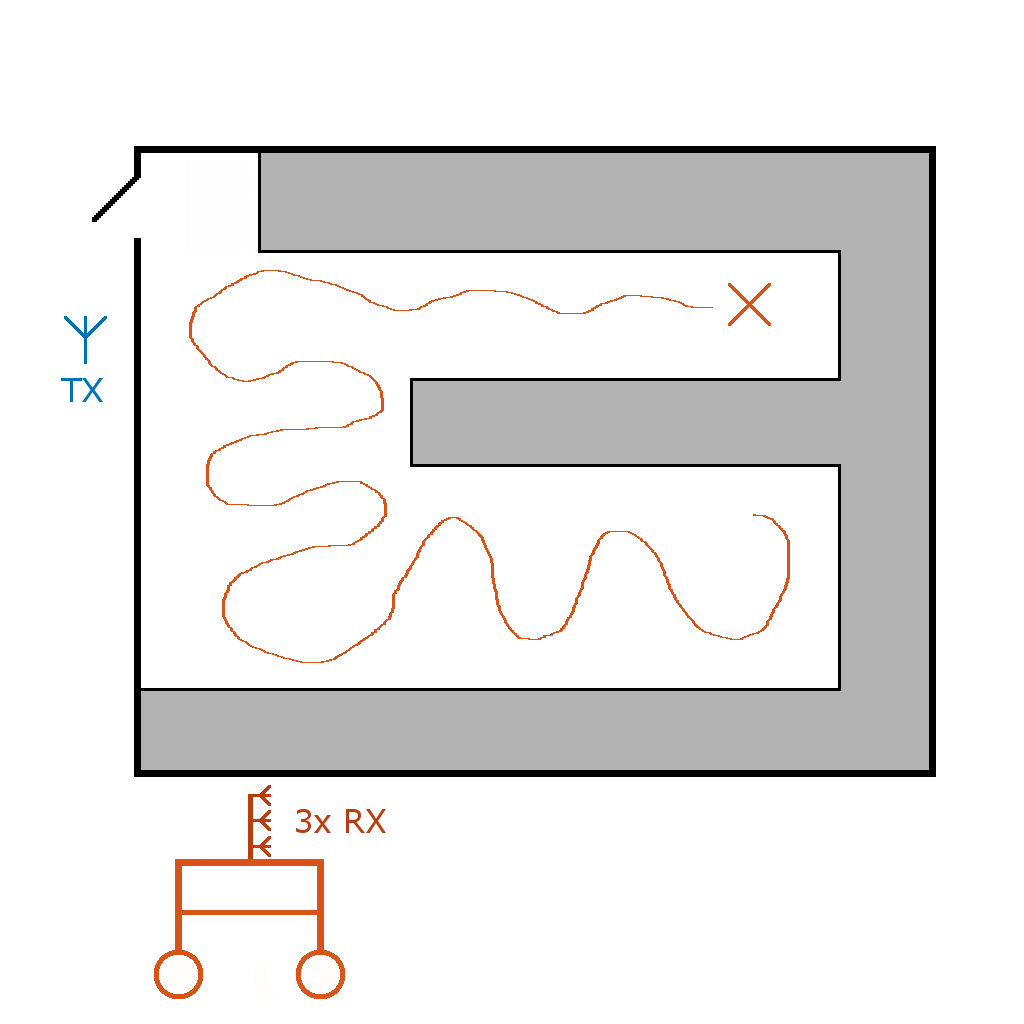
\includegraphics[width=0.75\textwidth]{figures/Gimp_figures/MeasSetup.png}
\caption{Sketch of the room}
\label{room sketch}
\end{figure}

The idea is to do a pilot test of the room. This is to obtain the pathloss $L$ and the delay spread of the room $\sigma_\tau$. With these values we can find the coherence bandwidth $B_c$ and the fading gain can be calculated. 
We suspect that since this is a multipath NLOS setup the delay spread and pathloss will be very similar across the room. But as a precaution the rooms pathloss and delay will be measured in a close,mid and far region from the doors where the signal originates. When the measurements are ongoing there will be some loss associated with body loss of the handsome scientist and clutter in the environment. This will give more multipath reflections compared to a a empty room.
\todo {read and rewrite to proper English}

With the pilot test done the full measurement can begin. This will use the same setup as for the pilot test, but with three reviver antennas measuring in parallel and different settings on the VNA. Given the results of the pilot test the amount of samples the sweep will obtain in frequency $N_f$ can be terminated. With this the amount of samples in space can be found to get a total of $4.04 \cdot 10^6$ samples.



\subsection{equipment}
\label{equip}
Keysight PNA N5527A 4-port VNA with parallel measurements and supports a frequencies from 10MHz to 67 GHz. The sweep data will me saved to a USB.

Cables used have a loss of $0.5dB per m$ 
Splitter to separate the signal to two TX antennas and point towards the doors for more equal distribution of signal.
N5527A has a $-119dB$ noise floor without averaging with a 10Hz $IF_{bw}$ at 1-10GHz. The dynamic range of the VNA becomes:

\begin{equation}
DR = P_{tx}-119dBm 
\label{NFvna}
\end{equation}

Antenna array 4Ghz $f_c$ With $>0.4 \lambda$ spacing.
\todo {pictures of antennas}

%The most important part of the setup is the equipment and how they are connected. The R\&S Spectrum Analyser (model FPL9KHz-6GHz) is the center of the setup. This is the receiver of our system and gives us a readout of the spectrum in terms of power (dBm) and frequency (Hz). The two main setting on the Spectrum analyser is IF filter bandwidth and resolution. These two values gives us a sweep time.
\subsection{Specifications}
In chapter 1 all the needed factors has been discussed. Now when the setup is designed it's important to set specifications.
\begin{table}[H]
\centering
\caption{Some example specifications}
\label{final_specs}
\begin{tabular}{|l|l|l|l|}
\hline
Number of samples needed         & N           & 4.04 million   & $4.04 10^6$        \\ \hline
Center Frequency                 & $f_c$       & 4Ghz           & $4 \cdot 10^9$     \\ \hline
Wavelength                       & $\lambda$   & 10cm           & 0.075m               \\ \hline
Coherence freq                   & $\Delta f$  & 3MHz           & $3 \cdot 10^6$     \\ \hline
Dynamic range                    & DR          & 98dB           & $2\cdot 10^10$             \\ \hline
Antenna diversity                & $A_{div}$   & 1x3            & 3                  \\ \hline
Intermediate frequency bandwidth & $IF_{BW}$     & 10KHz          & $10 \cdot 10^3$ \\ \hline
\end{tabular}
\end{table}
\section{Total Dynamic range}
Given \autoref{eq:path_loss} and the VNA specification given in \autoref{equip} we can find the total received power seen in the measurements and calculate the total dynamic range needed given the margin in \autoref{SNR_margin}:
\begin{equation}
L = 20log (4000MHz) + 28 \cdot log(5)-28 = 63.61dB \approx 64dB
\end{equation}

\begin{equation}
Noisefloor_{tot} = 64dB - 30dBm + 64dB = 98dBm 
\end{equation}
We assume that the noise floor of the \gls{VNA} scales linearly with a increased $IF_{BW}$. This would mean that a $IF_{BW}$ on the \gls{VNA} can be increased by:
\begin{equation}
\begin{split}
&= IF_{BW} = 119dB-98dB = 21dB \\
           &= 10Hz \rightarrow 20dB \rightarrow 1kHz
\end{split}
\end{equation}
\section{Sweep Time}
Since the \gls{VNA} can do segmented sweeps the sweep time is mostly dependant on the number of points and $IF_BW$.
The Keysight PNA N5527A gives the following sweep times for a 201 point with different $IF_BW$ \citep{Key_PNA}.

\begin{table}[H]
\centering
\caption{$IF_{BW} \ vs \ sweep time$}
\label{my-label}
\begin{tabular}{l|l}
\hline
$IF_BW${[}Hz{]} & Sweep time {[}ms{]} \\
10              & 17834               \\
100             & 1825                \\
300             & 641                 \\
1000            & 223                 \\
3000            & 72                 
\end{tabular}
\end{table}


There is also some overhead for saving the data.
\subsection{Total Time}
Let's use example where we can use a 1kHz $IF_BW$ a
\begin{equation}
T_{sweep total} = 223ms
\end{equation}
This means that every 223ms we have to move $\frac{\lambda}{2}$ this gives a relative velocity of:
\begin{equation}
\frac{0.0375m}{0.223s} = 0.17 m/s
\end{equation}
This is under the $1m/s$ value found in \autoref{min_vel}
and total time for moving 5 meters $\approx 30s$.
and with the speculated 80000 samples per 5 meter walk(200 samples in frequency). we need around:
\begin{equation}
\frac{4.04 \cdot 10^6}{80000} = 50.5 walks
\end{equation}
or around 25 minuets of measurement given 55.5 walks and 30s per walk and no wait time.
\section{Analysing raw data}

\todo {Write general about that to do with the data. How to obtain the fading gain. Running average, overall pathloss, close,mid,far region.}

\section{Analysing fading gain}
From the fading gains, gathered from the measurements, will now be compared to the theoretic values, that was expected, if the real world behaved like Rayleigh fading. With $4.04 \cdot 10^6$ measurements, the confidence level should be 90\% with an interval a $\pm 1dB$ at $10^{-5}$ level.

\section{Results}